\documentclass[a4paper]{article}
\usepackage{graphicx}
\usepackage{hyperref}
\usepackage{float}

\begin{document}

\begin{titlepage}
\title{Analyzing Unoccupied Setback Effectiveness and Prevalence}
\author{
	Jay Herron
	\and
	\url{https://github.com/NeedleInAJayStack/RTEM-Hackathon\_2022}
}
\date{\today}
\maketitle
\end{titlepage}

\section*{Executive Summary}

\paragraph{}
This document proposes two building-wide electric consumption KPIs: \textbf{Unoccupied Turndown Factor} and \textbf{Occupied Duration Factor}, which measure the effectiveness and prevalence of unoccupied setbacks respectively. It demonstrates that these KPIs can be used to identify buildings that may be able to reduce energy consumption by improving their unoccupied operation.  Finally, it asserts that this approach can be used across nearly every building in every geographic location, as long as the building's electric consumption varies with human occupancy.

\pagebreak

\section{Introduction}

\paragraph{}
The primary function of most buildings is to provide a comfortable environment for the occupants. As such, the majority of the energy use of a building is devoted to heating, cooling, ventilating, powering, and lighting the building for occupants. When these occupants leave, however, the need to provide many of these services is drastically reduced, and energy is wasted if the systems continue operating as if the space was still occupied. Ensuring quality unoccupied operation requires either sensor installation, integration, programming, and maintenance or ongoing efforts to adjust and maintain zone schedules. Since these efforts are error-prone, ensuring good unoccupied setbacks is typically the most cost effective energy savings opportunity in existing buildings.

\paragraph{}
This document proposes a set of key performance indicators (KPIs) and an analysis framework to identify and prioritize energy reduction through unoccupied setbacks. They identify opportunities to significantly reduce energy usage in a building by making basic changes to its unoccupied operation, typically by improving occupancy detection or modifying zone air temperature setpoints, minimum discharge air flow setpoints, or lighting status based on occupancy. These KPIs are applicable to nearly any building in any location using any HVAC system, as long as the building's electric consumption varies with human occupancy.

\section{Use Case and Demonstration}

\subsection{Approach}

\paragraph{}
The proposed framework requires only a single whole-building electric consumption point, recorded at hourly frequencies or faster. The energy consumption is then cleaned by removing meter rollover artifacts, aligning time-stamps to a consistent frequency, and interpolating missing values. Next, the values are dis-aggregated if usage is represented by a monotonically increasing counter, and finally the history is passed through a filter to remove outliers. At this point, the data is clean, normalized, and ready for analysis

\paragraph{}
The cleaned data is split into weekly periods, each of which is passed through a k-means clustering algorithm\footnote{\url{https://en.wikipedia.org/wiki/K-means\_clustering}} that identifies 2 nodes: a high-usage cluster and a low-usage cluster. This results in a mapping between each historical observation and whether it belongs in the high or low group, as well as average values for these high and low groups. In general, we interpret the high-usage period to be the occupied time in a building, and the low-usage period to be the unoccupied time.

\paragraph{}
From these results, two meaningful weekly KPIs can be computed:
\begin{enumerate}
\item{\textbf{Unoccupied Turndown Factor}: The high-usage cluster value divided by the low-usage cluster value. Scaled from 0 to 1, lower values indicate more effective unoccupied setbacks. Lower is better from an energy reduction standpoint.}
\item{\textbf{Occupied Duration Factor}: The amount of time the building was in a high-usage state, divided by the total time in the KPI period. Scaled from 0 to 1, lower values indicate more prevalent unoccupied setbacks, in terms of time.  Lower is better from an energy reduction standpoint.}
\end{enumerate}

\paragraph{}
This simple approach offers several distinct advantages. First, the data requirements are extremely low; only a single historical point is required. Of the 230 buildings in the Real Time Energy Management (RTEM) dataset from New York State Energy Research and Development Authority (NYSERDA), 99 have \textit{Electric Consumption} points, making it the 5th most prevalent point type behind only  \textit{Virtual}, \textit{Zone Temperature}, \textit{Outside Air Temperature}, and \textit{Status}. Second, it is widely applicable. The analysis process is not impacted by the type of building, the pattern of occupancy throughout the week, the location of the building, or the type or complexity of the equipment systems within the building. Since no assumptions are made on the time of occupancy, it functions as well on irregularly occupied buildings (like community centers or theaters) as on regularly occupied buildings (like commercial office buildings or retail). Third, it delivers actionable results. Even the most primitive control systems offer features for modifying building operation according to occupancy.

\subsection{Usage}

\paragraph{}
These KPIs alone do not scale according to energy usage, so they are best used as part of a top-down Energy Use Intensity (EUI) based analysis. For example, if comparing buildings within a portfolio, the EUI could be used to determine the worst-performing facilities, and then the KPIs above could be used to determine whether these facilities would benefit from improving the unoccupied operation.

\paragraph{}
The KPIs suggest different actions:
\begin{itemize}
\item{A large Unoccupied Turndown Factor suggests that unoccupied operation should be investigated. When unoccupied, zone air temperature setpoint deadbands should widen significantly, minimum discharge airflow setpoints and outside air flow setpoints should be set as low as possible, and lights should be turned off. This KPI may also suggest that there are areas of the building that never enter an unoccupied state.}
\item{A large Occupied Duration Factor suggests that occupancy scheduling and detection systems should be investigated. Of course, unoccupied energy saving measures must conform to each building's unique occupancy patterns. However, if occupancy is based on a schedule, that schedule should be checked to ensure that it matches actual occupancy patterns. If occupancy is detected using a sensor, the sensors should be validated for correct operation.}
\end{itemize}

\paragraph{}
While a KPI value on a particular building during a particular week is meaningful, KPIs are typically most useful when they are compared between entities or over time. A building with a large KPI value compared to its peers, or with a KPI value that increases over time may provide context on what constitutes a large KPI value.

\subsection{Results}

\paragraph{}
See KPI results for each building in Table 1 of the Appendix.

\subsection{Example Analysis}

\subsubsection{Building 188}

\paragraph{}
Building 188 and Building 165 are identically sized commercial retail spaces with similar occupied electricity consumption. However, Building 188 has an average unoccuiped turndown factor of 0.424 while Building 165 has a value of 0.147. Figure 1 compares the total consumption of these two buildings over a representative week in June 2019 and shows that Building 188 has significantly higher usage during unoccupied times, as predicted by the higher unoccupied turndown KPI value.

\begin{figure}[H]
\centering
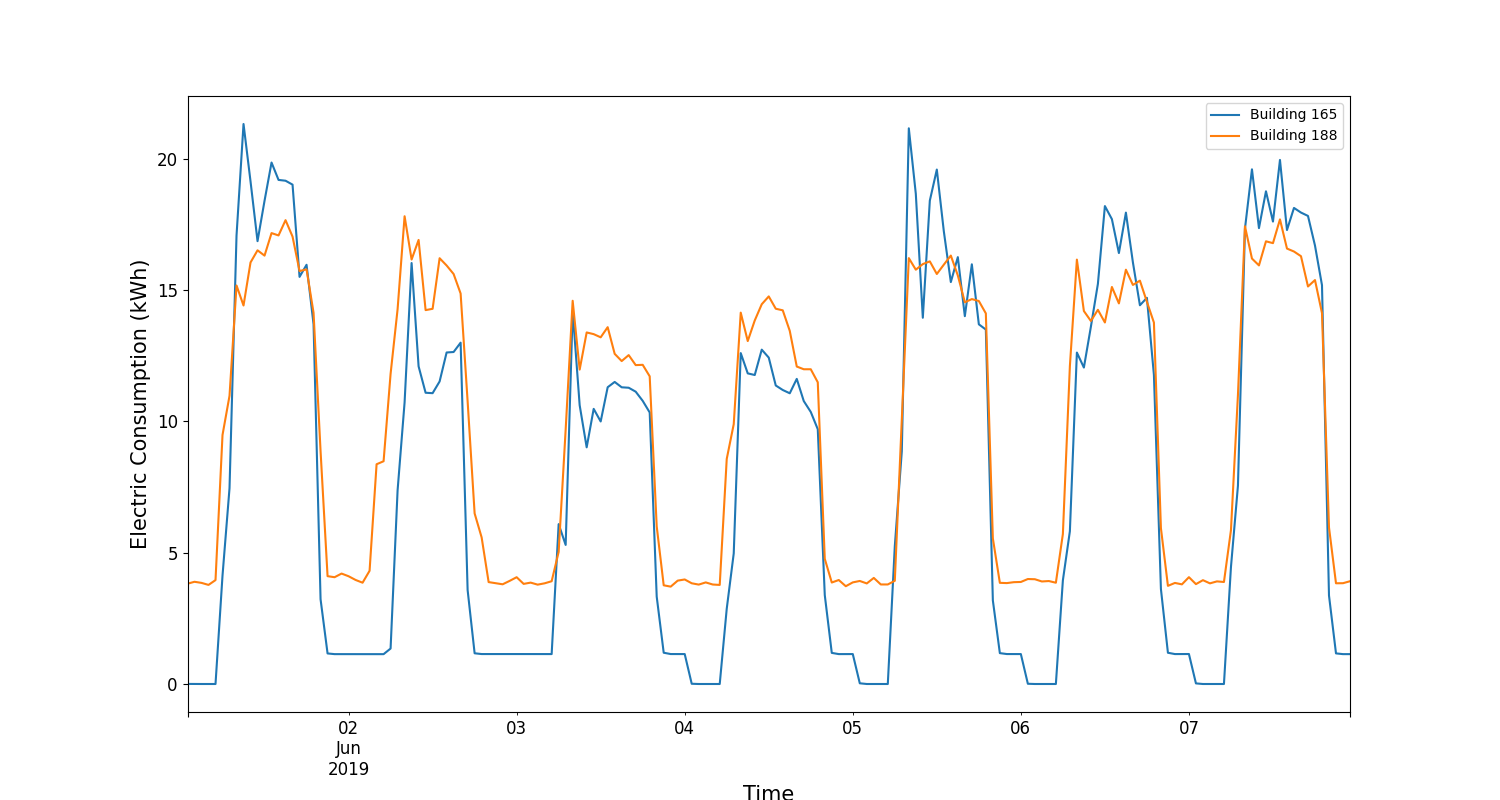
\includegraphics[width=.9\columnwidth]{./images/188v165_Turndown.png}
\caption{Building 165 and 188 total electric consumption in kilowatt-hours from June 1 to June 7, 2019}
\end{figure}

\paragraph{}
Since these facilities have HVAC submetering, we can dis-aggregate the whole-building electricity consumption. Figure 2 shows the submeter HVAC electric consumption for each building over the same time period. The nighttime HVAC consumption in Building 188 is much lower than the total consumption, indicating that it is unrelated to the HVAC equipment and is likely related to light or plug loads.

\begin{figure}[H]
\centering
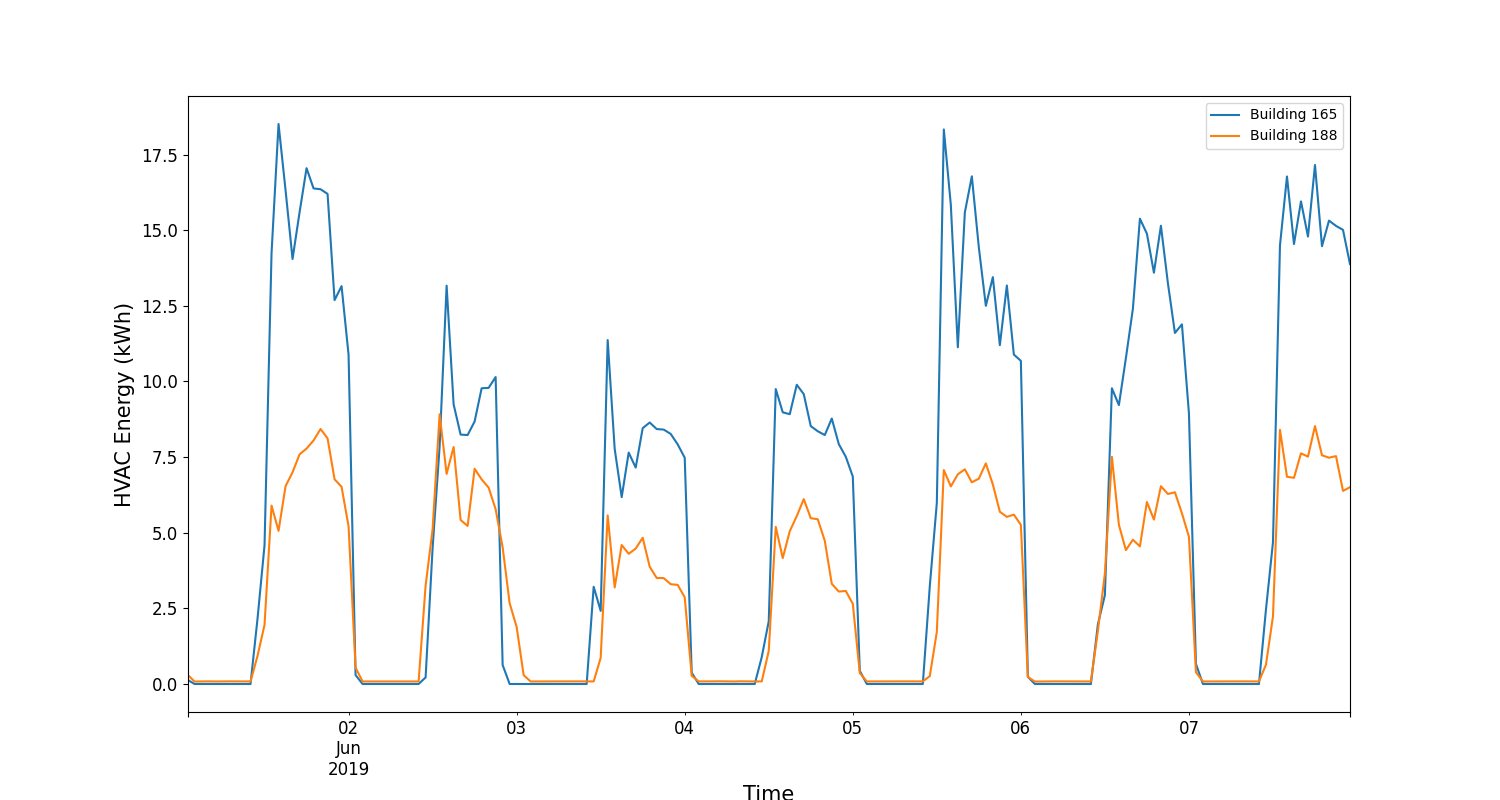
\includegraphics[width=.9\columnwidth]{./images/188v165_Turndown_HVAC.png}
\caption{Building 165 and 188 HVAC electric consumption in kilowatt-hours from June 1 to June 7, 2019}
\end{figure}

\paragraph{}
If Building 188 is able to achieve a turndown equivalent to that of Building 165, the KPIs suggest that its energy consumption will be reduced by about 11,500 kilowatt-hours (kWh) per year, which is roughly 16\% of its total yearly energy usage.

\subsubsection{Building 275}

\paragraph{}
Building 275 and 393 are both large office buildings. Building 393 has more than twice the square footage and three times the occupied electrical consumption of 275. However, with an unoccuiped turndown factor of 0.821, Building 275 has much less effective unoccupied setbacks than Building 393, whose factor is 0.336. Figure 3 shows the total electric consumption for both buildings for a week in early March 2020, and illustrates that Building 275 has much less variance in consumption between daytime to nighttime hours.

\begin{figure}[H]
\centering
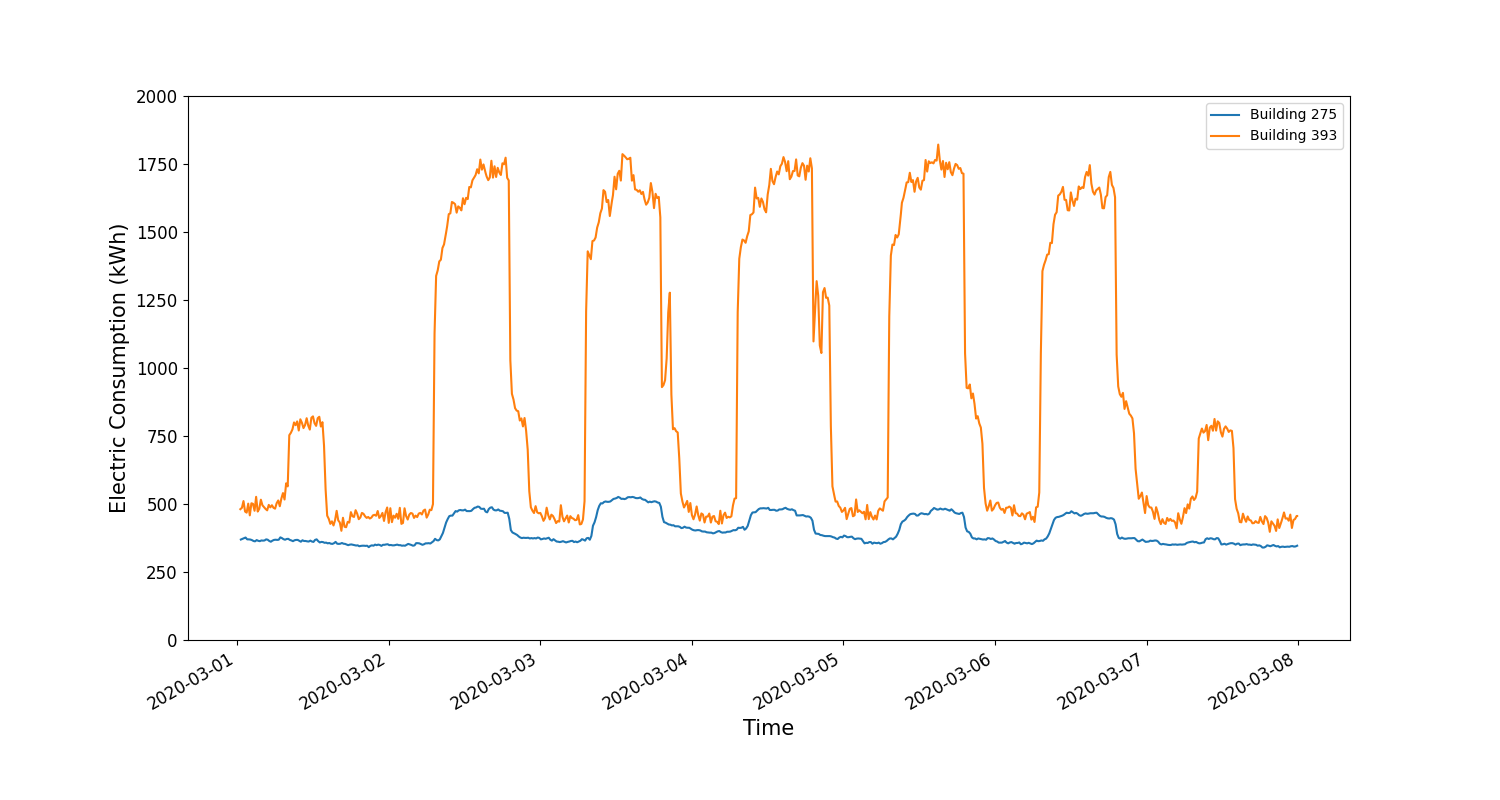
\includegraphics[width=.9\columnwidth]{./images/275v393_Turndown.png}
\caption{Building 275 and 393 total electric consumption in kilowatt-hours from March 1 to March 7, 2020}
\end{figure}

\paragraph{}
If Building 275 was able to achieve the same unoccupied turndown factor as 393, which is not unusual in the commercial office group, it would reduce its total energy use by an estimated 36\%. Extrapolating from the 6 months of available energy usage data, this would result in savings of 5,000,000 kWh or \$750,000 of reduced consumption charges per year, assuming an average electric rate of 15¢/kWh.

\subsubsection{Building 390}

\paragraph{}
Building 390 is a food and beverage facility, with a large occupied duration factor of 0.798. Figure 4 shows the total electrical consumption over a week in July 2019 and indicates that the daily high-usage period typically spans 20 hours, from 4AM to midnight.

\begin{figure}[H]
\centering
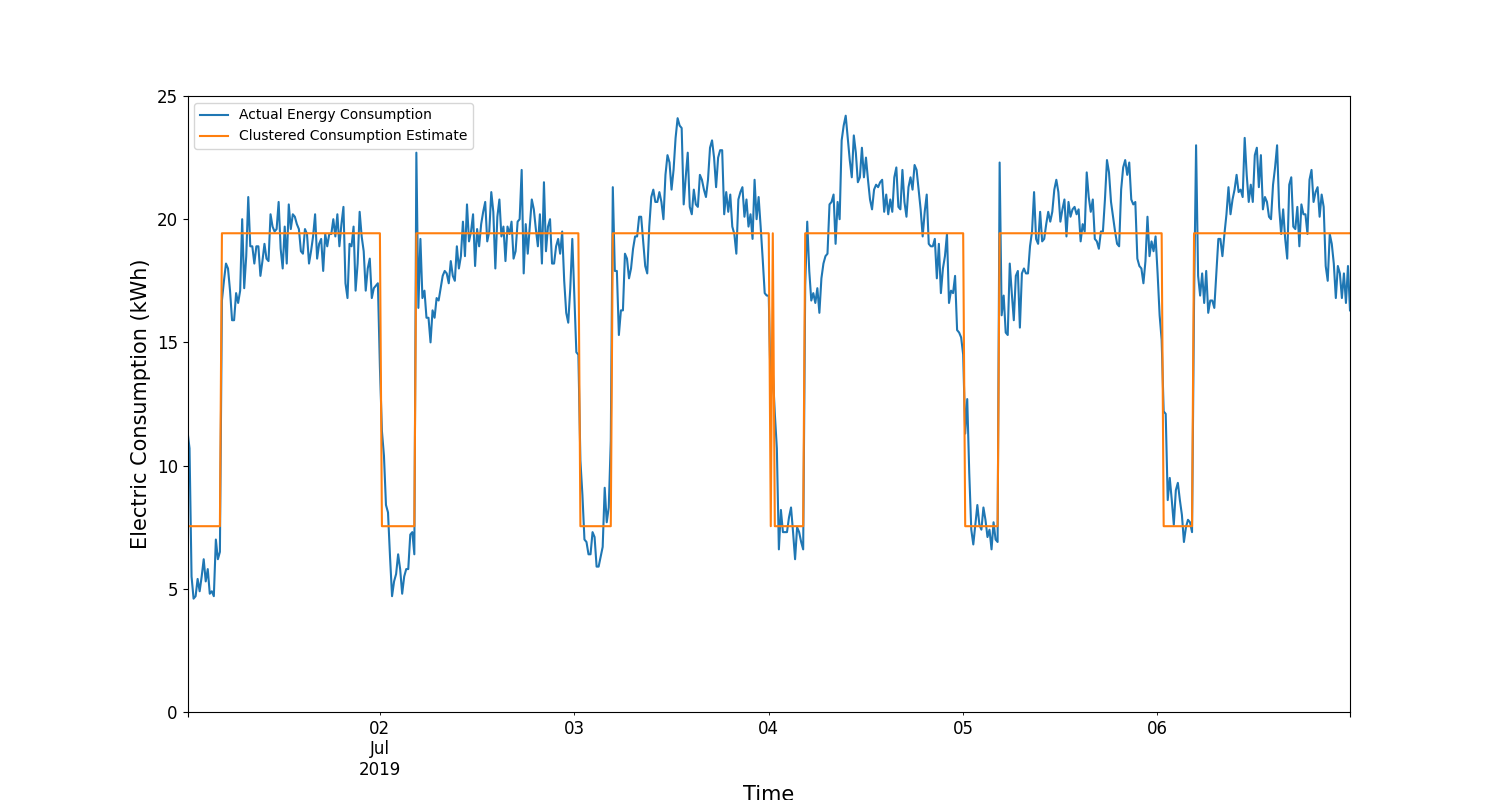
\includegraphics[width=.9\columnwidth]{./images/390_Duration.png}
\caption{Building 390 actual and clustered electric consumption in kilowatt-hours from July 1 to July 7, 2019. The clustered value shows whether the consumption at a particular timestamp was placed in a high or low usage cluster.}
\end{figure}

\paragraph{}
There are certainly food and beverage facilities that keep these hours as staff prepare in the morning and clean at night. However a quick investigation could determine if the consumption profile reflects actual occupancy schedules. If not, and the building could be run in an unoccupied mode even just 2 additional hours each day, modifying the HVAC schedule would save nearly 5\% of this building's total energy consumption.

\section{Market Characterization}

\paragraph{}
These KPIs are applicable to any party interested in reducing the energy of a specific building or fleet of buildings. This includes portfolio energy managers, facility managers, individual building owners, energy-efficiency consulting firms, and utility energy reduction programs. The results computed are applicable for every building type in every geographical location, as long as building electric energy use is impacted by occupancy. Due to the open-source license of the code and the prevalence of Python language support, the KPI computation could be integrated into an enormous variety of software applications or presentation systems.

\section{Market Adoption and Impact}

\paragraph{}
Analytics are most effective when they provide owners and operators with as much guidance as possible. To accomplish this, the ideal market strategy would be for NYSERDA to use these KPIs to identify buildings with large energy savings opportunities, and offer guidance to the relevant owners or facilities teams on how to achieve these savings. If this is not feasible, NYSERDA could create a real-time dashboard that allows owners and operators to see the KPIs for their building and how they perform compared to their peers. Detailed descriptions of how to achieve unoccupied energy savings should accompany the KPI values. If the information provided is high quality and drives energy reduction, other building owners will seek to join the RTEM dataset, expanding the total RTEM System market.

\section{Decarbonization through Electrification}

\paragraph{}
Energy conservation is a win-win with regards to decarbonization. By improving building energy efficiency, not only is a building's carbon footprint reduced in the short term, but transitioning it to renewable energy sources becomes more feasible. In order to maximize ongoing investments in renewable power generation, there should be simultaneous efforts to implement high-value low-cost energy conservation measures in existing buildings. Whether due to occupancy schedule changes, temperature setpoint overrides, poor ventilation adjustments, or various other issues, many buildings use more energy than necessary during unoccupied hours making unoccupied energy reductions one of the most effective means to reduce total energy consumption. The provided KPIs are able to identify this opportunity by detecting when the unoccupied operation is poor, or when the occupied period lasts longer than normal.

\section{Ease of Implementation}

\paragraph{}
The results tabulated in the Appendix and available in the associated GitHub repository are an aggregation of these KPIs over the entire history of all possible buildings in the RTEM dataset. Re-computation is as easy as running the scripts provided in the GitHub, and currently takes only a few minutes on commodity hardware. As the RTEM dataset expands, these weekly KPIs can be automatically computed on new data. By default, these scripts fetch the entire history for a given building, so integrating new data on existing buildings is as simple as re-running the script.

\paragraph{}
Adding new buildings to the dataset is also easy, but not automatic. Unfortunately, the modeling of electrical metering within the RTEM dataset is not sophisticated enough to determine which points represent whole-building usage. For example, given a site with multiple electric consumption readings, it is not denoted whether a specific reading is a subset of another or is fully separate. Top level consumption readings are not differentiated from low-level submeters. Due to this, the final list of points used within the analysis was manually revised to determine which points (or collection of points) represented each building as a whole. New buildings must have their whole-building electricity consumption points added to this list.

\paragraph{}
Project Haystack models metering trees using the \texttt{submeterOf}\footnote{\url{https://project-haystack.org/doc/lib-phIoT/submeterOf}} tag, and denotes top-level metering using a \texttt{meterScope}\footnote{\url{https://project-haystack.org/doc/lib-phIoT/meterScope}} tag. Brick Schema models building-level meters with a \texttt{Building Meter}\footnote{\url{https://brickschema.org/ontology/1.2/classes/Building\_Meter}} class. Adding these concepts into the RTEM ontology would improve future automation efforts.

\paragraph{}
This proposal does not recommend a particular presentation format. The proposed KPI data can support an enormous variety of presentation options ranging from interactive, realtime dashboards to periodic PDF reports to HTML-formatted emails. The particular presentation format should be chosen based on what is most effective in communicating with a particular market segment.

\section{Use of Open Data Sources}

\paragraph{}
The only data source used within this demonstration was the NYSERDA RTEM database, and the solution presented would continue to be effective as this dataset grows across both time and buildings. That said, targeted partnerships could accelerate this effort. Partnerships with utilities like New York State Electric and Gas or utility data providers like Urjanet\footnote{\url{https://urjanet.com/utility-data/}} could drastically increase the number of buildings that have high-resolution total building consumption information. Alternatively, partnerships with data collection companies like Obvius Acquisuite\footnote{\url{http://www.acquisuite.com}} could allow data collection without requiring coordination with utilities. 


\section{Additional Applications}

\paragraph{}
The clustering approach shown in this document is not specific to whole-building electric energy use. It could potentially be applied to:
\begin{description}
\item[Other whole-building utilities]{Whole-building natural gas, chilled water, or steam consumption also typically have historical profiles correlated to building occupancy. A nearly identical analysis could be performed to determine whether occupancy setbacks produce good turndowns in these other utilities as well.}
\item[Submetering]{If submetering data is available, an unoccupied setback analysis could be performed on each submeter to determine which areas contribute to poor performance at the whole building level. These submeters might cover categories like HVAC, plug, and lighting, or they might cover different tenant zones. The setback analysis approach in this document would apply well to either configuration.}
\item[Non-energy points]{The effectiveness of occupancy setbacks can also be analyzed from low-level non-energy points, such as zone air temperature heating/cooling setpoints, or minimum VAV discharge airflow setpoints. These points may be analyzed via clustering to determine if they change significantly during unoccupied times and for how long. Those results can be used to determine which specific areas of a building contain opportunities for unoccupied setback energy savings.}
\end{description}

\section{Conclusion}

\paragraph{}
This document presents a strategy for analyzing the effectiveness and prevalence of unoccupied setbacks by using a clustering algorithm on historical whole-building electrical consumption. It outlines the KPIs that can be calculated from the consumption history, and demonstrates how they can be used on real-world data from the RTEM dataset. Finally, it discusses the feasibility of a wider implementation and relevant market considerations.

\paragraph{}
Energy conservation is the most cost-effective means of decarbonization. Of course, investments should be made in converting fossil fuel-based energy production to renewables. However, in the meantime, we must also make sure that our existing infrastructure is working as efficiently and effectively as possible. Poor unoccupied operation is often the largest opportunity for building energy reduction that does not require a major capital investment. We need automated, visible metrics that ensure that these opportunities are being fulfilled now and will continue to be fulfilled in the future.

\pagebreak
\section{Appendix}

\begin{table}[H]
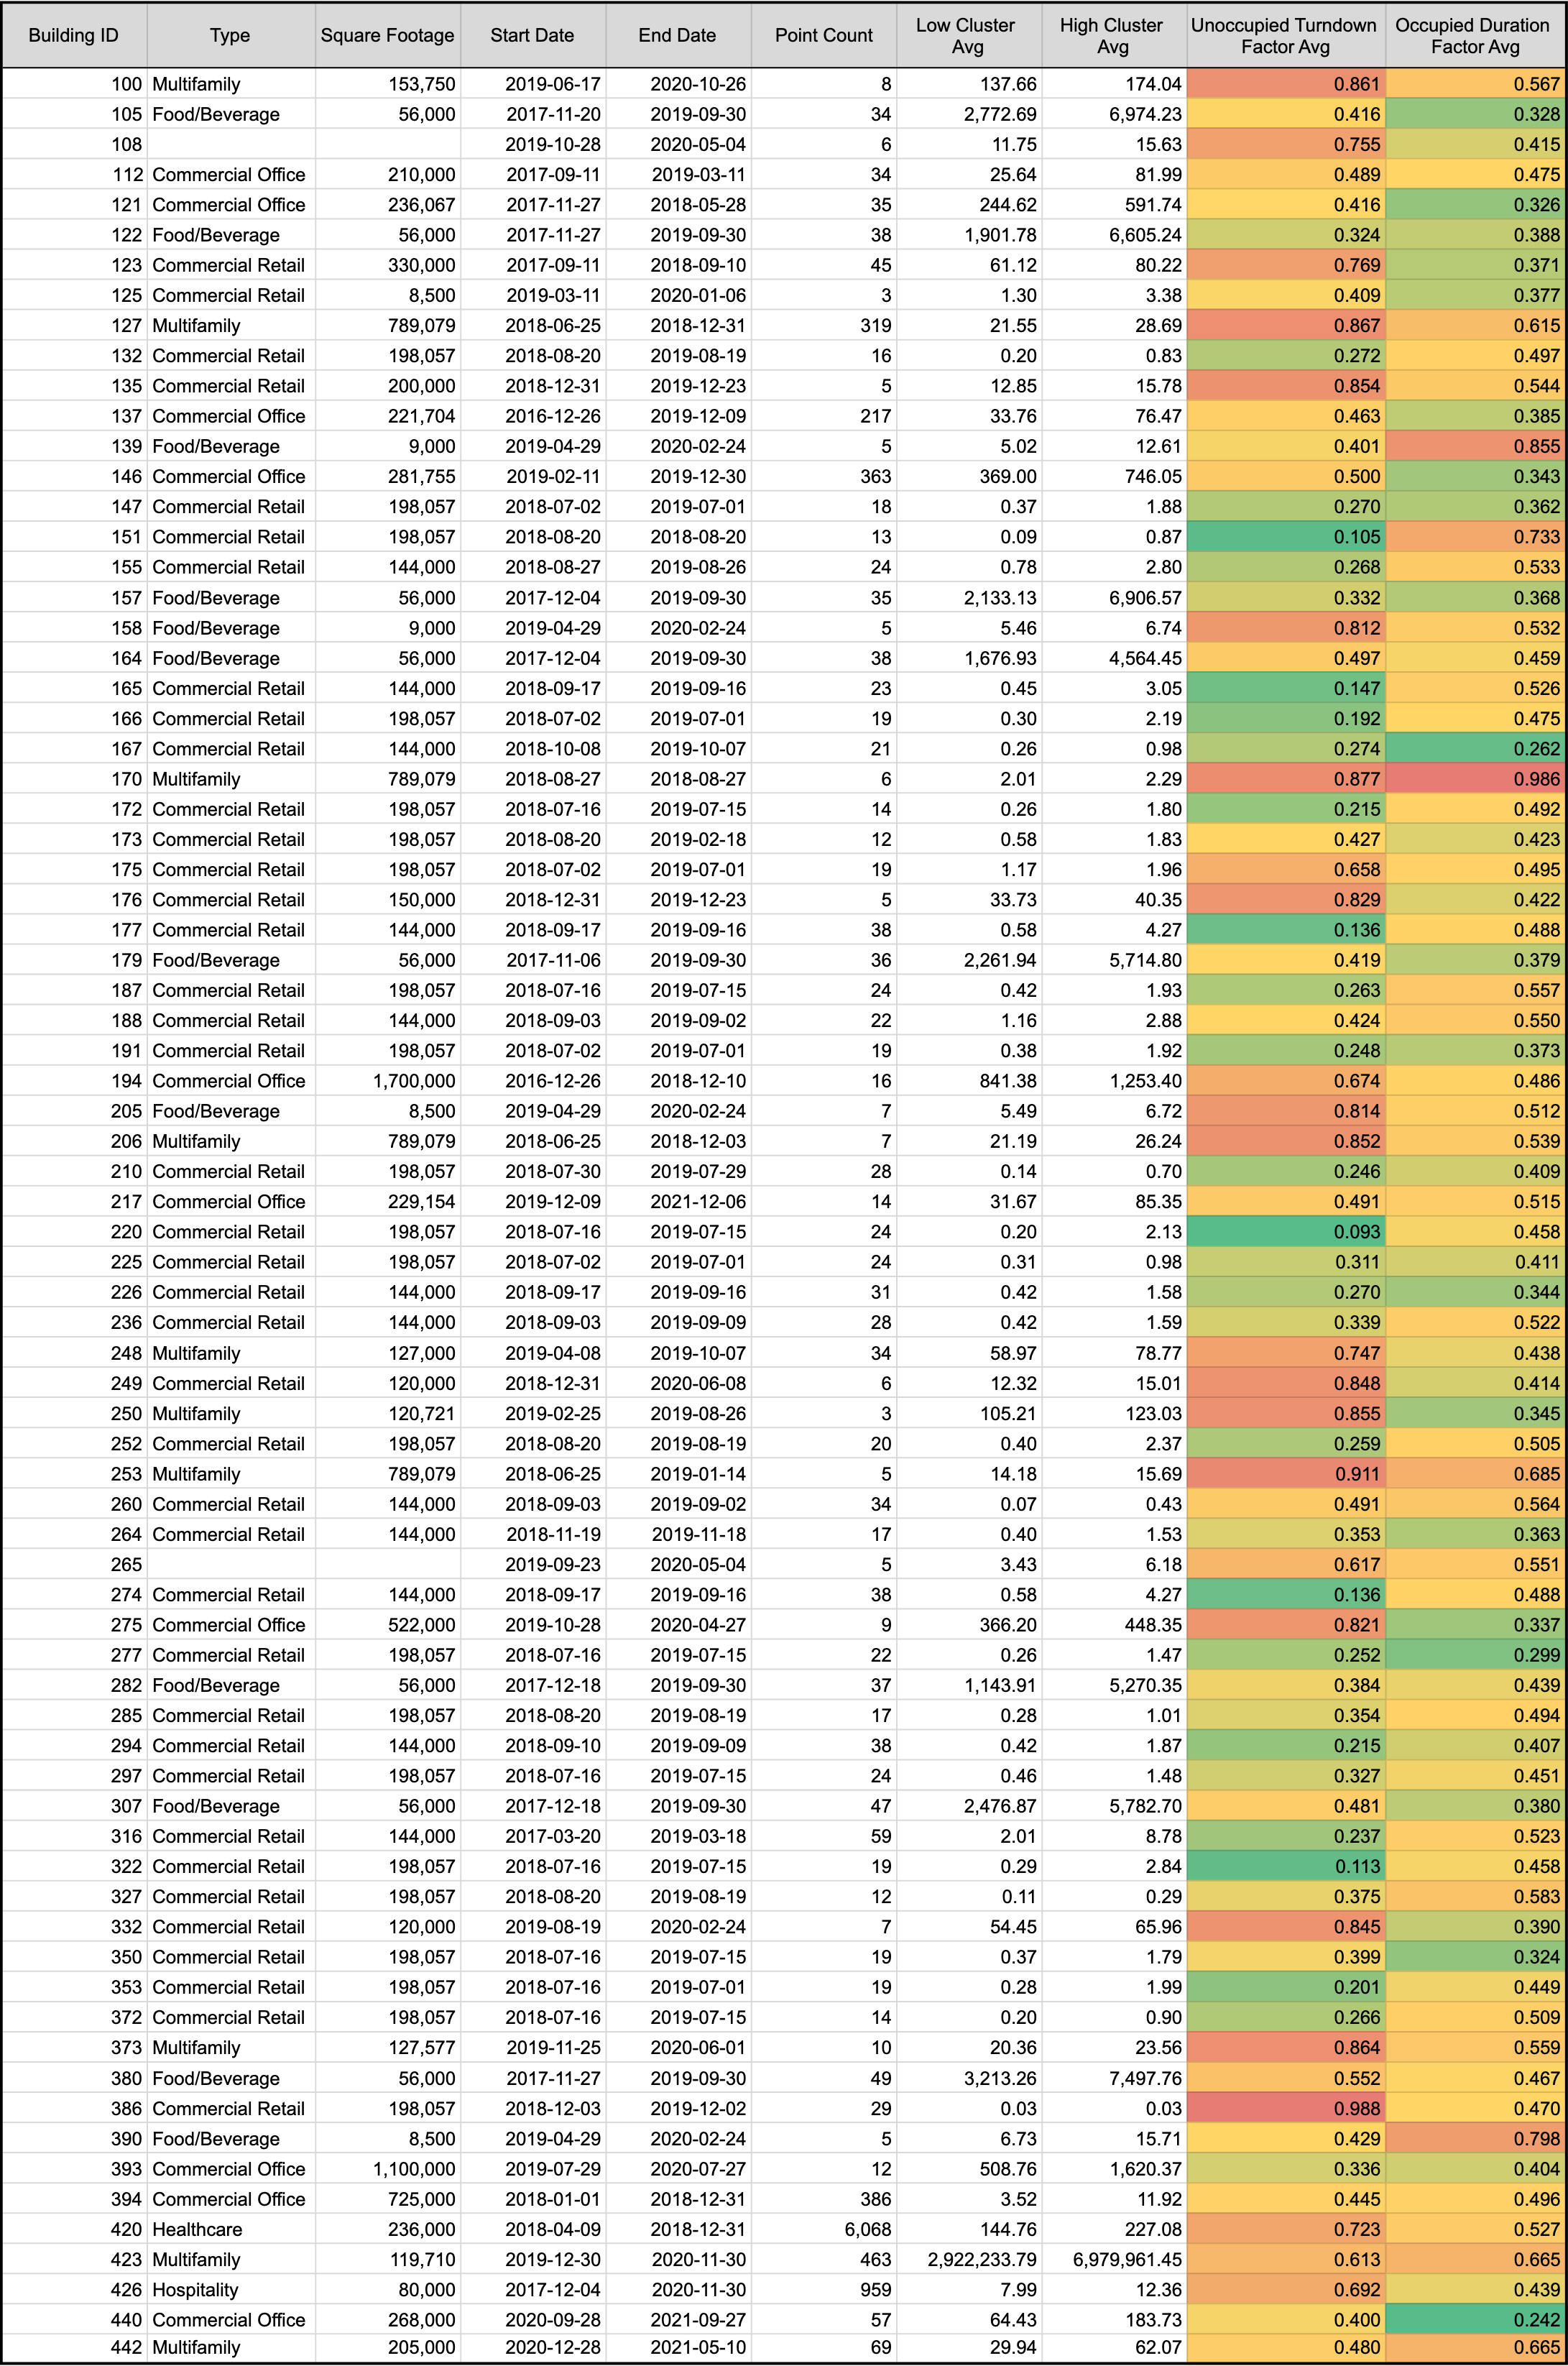
\includegraphics[width=0.9\columnwidth]{./images/KPI_Result_Table.png}
\caption{Buildings with associated KPI values computed across the building's entire historical dataset}
\end{table}


\end{document}